\documentclass[a4paper,10pt,DIV=14]{scrartcl}
\usepackage{graphicx}
\usepackage[utf8]{inputenc} % korrekte Darstellung von Umlauten u. Sonderzeichen
\usepackage[ngerman]{babel} % Sprachpaket, ngerman = neue deutsche Rechtschreibung
\usepackage{amsmath} % Setzen mathematischer Formeln
\usepackage{titlesec}
\usepackage{float}
\usepackage{caption}
\usepackage{fancyvrb}
\usepackage{siunitx}
\usepackage{booktabs}
\usepackage{enumitem}
\usepackage{gensymb}

\usepackage{tabularx}
\newcolumntype{L}[1]{>{\raggedright\arraybackslash}p{#1}} % linksbündig mit Breitenangabe
\newcolumntype{C}[1]{>{\centering\arraybackslash}p{#1}} % zentriert mit Breitenangabe
\newcolumntype{R}[1]{>{\raggedleft\arraybackslash}p{#1}} % rechtsbündig mit Breitenangabe

\newcommand{\gqq}[1]{\glqq{}#1\grqq{}}
\newcommand{\gq}[1]{\glq{}#1\grq{}}
\newcommand{\dg}[1]{#1^\circ}

\renewcommand{\thesection}{Aufgabe \arabic{section}:}
\renewcommand{\thesubsection}{\alph{subsection})}
\titleformat*{\subsection}{\normalfont\fontfamily{phv}\fontsize{12}{15}\selectfont}


\captionsetup[figure]{labelformat=empty}


\begin{document}

\title{Graphische Datenverarbeitung WS17/18 \\ Theorieübung 1}
\author{
  Salmah Ahmad (2880011)
  \and
  Markus Höhn (1683303)
  \and
  Tobias Mertz (2274355)
  \and
  Steven Lamarr Reynolds (1620638)
  \and
  Sascha Zenglein (2487032)
}

\maketitle

\section{Pipeline}

\subsection{Aus was besteht der Input der Pipeline?}
Der Input der Pipeline besteht aus einer gegebenen Szenenbeschreibung.


\subsection{Zum Input gehören unter anderem \gqq{Objekte}. In welcher Form sind konkrete \gqq{Objekte} im Input gegeben?}

\begin{itemize}[itemsep=0pt]
	\item (virtuelle) Kamera
	\item Dreidimensionale Objekte
	\item Lichtquellen
	\item Beleuchtungsalgorithmen
	\item Texturen
	\item ...
\end{itemize}


\subsection{Was ist der Output der Pipeline?}
Der Output der Pipeline ist ein 2D Bild der gegeben Szenenbeschreibung.


\subsection{Weshalb ist eine Pipeline die aus $n$ Abschnitten besteht (theoretisch) $n$-mal schneller als eine Pipeline mit nur einem Abschnitt?}
Bei einer Pipeline mit $n$ Abschnitten kann eine parallele Verarbeitung durchgeführt werden.


\subsection{Weshalb ist die Pipeline Geschwindigkeit vom Bottleneck abhängig? Wieso warten die anderen Pipeline-Abschnitte bis der Bottleneck-Abschnitt fertig ist?}
Der Bottleneck-Abschnitt ist der langsamste der Pipeline. Die Berechnung eines Frames basiert auf den Ergebnissen der vorausgegangenen Pipeline-Abschnitte. Daher ist die Geschwindigkeit der Pipeline abhängig vom langsamsten Verarbeitungsschritt.


\section{Model \& View Transformation}

%\subsection{Stellen Sie die Gleichung $(x, z)^T = f(u,v)$ auf, die die $u, v$ Koordinaten in das Weltkoordinatensystem transformiert. Bestimmen Sie nun die Position der Szenenobjekte bezüglich des Weltkoordinatensystems.}
%
%$$f(u,v) = \begin{pmatrix}
%\cos(\alpha) & \sin(\alpha)  & r \cdot \cos(\alpha)  \\
%\sin(\alpha) & -\cos(\alpha) & -r \cdot \sin(\alpha) \\
%0            & 0             & 1                     \\
%\end{pmatrix} \cdot \begin{pmatrix} u \\ v \\ 1 \\ \end{pmatrix} $$
%
%Ergebnisse:
%\begin{itemize}[itemsep=0pt]
%	\item Sonne: $ (0, 0)^T $
%	\item Planet: $ (-2\sqrt{3}, -2)^T $
%	\item Mond: $ (2 - 2\sqrt{3}, -3)^T $
%\end{itemize}

\subsection{Stellen Sie die Gleichung $(x, z)^T = f(u,v)$ auf, die die $u, v$ Koordinaten in das Weltkoordinatensystem transformiert. Bestimmen Sie nun die Position der Szenenobjekte bezüglich des Weltkoordinatensystems.}

Um die Koordinaten des Planetenkoordinatensystems in das Weltkoordinatensystem zu transformieren, sind die folgenden Schritte notwendig:
\begin{enumerate}[itemsep=0pt]
\item Das Planetenkoordinatensystem muss so gedreht werden, dass die v-Achse entgegengesetzt zur z-Achse verläuft, also nach oben zeigt. Hierzu müssen Koordinaten um $270\degree - \alpha$ im Uhrzeigersinn oder $\alpha + 90\degree$ gegen den Uhrzeigersinn rotiert werden.
\item Danach müssen die Koordinaten an der u-Achse gespiegelt werden, sodass die v-Achse nun in Richtung der z-Achse zeigt.
\item Als letztes muss jeder Punkt um die aktuelle Position des Planeten im Weltkoordinatensystem verschoben werden.
\end{enumerate}

\newcommand{\rotangle}{\alpha + 90 \degree}
\begin{enumerate}[itemsep=0pt]
\item Die Rotationsmatrix für die beschriebene Rotation ist folgende:
\[
R = 
\begin{pmatrix}
\cos(\rotangle) & -\sin(\rotangle) \\
\sin(\rotangle) & \cos(\rotangle) \\
\end{pmatrix}
\]
\item Die Spiegelung an der x-Achse wird beschrieben durch die Multiplikation mit:
\[
M =
\begin{pmatrix}
1 & 0 \\
0 & -1 \\
\end{pmatrix}
\]

\item Die Translation wird durch die Addition mit 
\[
t= 
\begin{pmatrix}
\cos \alpha \cdot r \\
-\sin \alpha \cdot r \\
\end{pmatrix}
\]
beschrieben.
\end{enumerate}
Diese Operationen in der genannten Reihenfolge beschreiben die gesuchte Funktion $f(u,v)$, die folgendermaßen aussieht:
\begin{align*}
f(u,v) &= 
t + M \cdot R \cdot
\begin{pmatrix}
u \\
v \\
\end{pmatrix} \\
&= 
\begin{pmatrix}
\cos \alpha \cdot r \\
-\sin \alpha \cdot r \\
\end{pmatrix}
+ 
\begin{pmatrix}
1 & 0 \\
0 & -1 \\
\end{pmatrix}
\cdot
\begin{pmatrix}
\cos(\rotangle) & -\sin(\rotangle) \\
\sin(\rotangle) & \cos(\rotangle) \\
\end{pmatrix}
\cdot
\begin{pmatrix}
u \\
v \\
\end{pmatrix}
\\
&= 
\begin{pmatrix}
\cos \alpha \cdot r\\
-\sin \alpha \cdot r\\
\end{pmatrix}
+ 
\begin{pmatrix}
\cos(\rotangle) & -\sin(\rotangle) \\
-\sin(\rotangle) & -\cos(\rotangle) \\
\end{pmatrix}
\cdot
\begin{pmatrix}
u \\
v \\
\end{pmatrix}
\\
\end{align*}

Die Ergebnisse für die genannten Objekte sind:
\begin{itemize}
\item Sonne: Position: $(u,v)^T = (0,4)^T$ 
\begin{align*}
f(0,4) &=
\begin{pmatrix}
\cos 150\degree \cdot 4 \\
-\sin 150\degree \cdot 4 \\
\end{pmatrix}
+ 
\begin{pmatrix}
\cos 240\degree & -\sin 240\degree \\
-\sin 240\degree & -\cos 240\degree \\
\end{pmatrix}
\cdot
\begin{pmatrix}
0 \\
4 \\
\end{pmatrix}
\\
&=
\begin{pmatrix}
-2\sqrt{3} \\
-2
\end{pmatrix}
+ 
\begin{pmatrix}
2\sqrt{3} \\
2  \\
\end{pmatrix}
= \begin{pmatrix}
0 \\
0
\end{pmatrix}
\end{align*}
\item Planet: Position: $(u,v)^T = (0,0)^T$ 
\begin{align*}
f(0,0) &=
\begin{pmatrix}
\cos 150\degree \cdot 4 \\
-\sin 150\degree \cdot 4 \\
\end{pmatrix}
+ 
\begin{pmatrix}
\cos 240\degree & -\sin 240\degree \\
-\sin 240\degree & -\cos 240\degree \\
\end{pmatrix}
\cdot
\begin{pmatrix}
0 \\
0 \\
\end{pmatrix}
\\
&=
\begin{pmatrix}
-2\sqrt{3} \\
-2
\end{pmatrix}
+ 
\begin{pmatrix}
0 \\
0 \\
\end{pmatrix}
= \begin{pmatrix}
-2\sqrt{3} \\
-2
\end{pmatrix}
\end{align*}
\item Mond: Position: $(u,v)^T = (\cos\beta \cdot r_M, \sin\beta \cdot r_M)^T = (-\sqrt{3}, 1)^T$
\begin{align*}
f(-\sqrt{3}, 1) &=
\begin{pmatrix}
\cos 150\degree \cdot 4 \\
-\sin 150\degree \cdot 4 \\
\end{pmatrix}
+ 
\begin{pmatrix}
\cos 240\degree & -\sin 240\degree \\
-\sin 240\degree & -\cos 240\degree \\
\end{pmatrix}
\cdot
\begin{pmatrix}
-\sqrt{3} \\
1 \\
\end{pmatrix}
\\
&=
\begin{pmatrix}
-2\sqrt{3} \\
-2
\end{pmatrix}
+ 
\begin{pmatrix}
\sqrt{3} \\
-1  \\
\end{pmatrix}
= \begin{pmatrix}
-\sqrt{3} \\
-3
\end{pmatrix}
\end{align*}
\end{itemize}


\subsection{Bestimmen Sie, welche Translation und welche Rotation auf die Szene ausgeübt werden müssen, um die Kamera in den Ursprung zu verschieben und anschließend die Blickrichtung nach -z zu rotieren.}

\begin{itemize}
	\item Translation: $ \left(-2, -2\sqrt{3}\right)^T $
	\item Winkel: $ \arctan\left(\frac{2}{2\sqrt{3}}\right) = \dg{30} $
	\item Rotation: $ \begin{pmatrix}	\cos(\dg{30}) & -\sin(\dg{30}) \\ \sin(\dg{30}) & cos(\dg{30}) \\ \end{pmatrix}
	= \begin{pmatrix} \frac{\sqrt{3}}{2} & \frac{1}{2} \\ \frac{1}{2} & \frac{\sqrt{3}}{2} \end{pmatrix} $
\end{itemize}


\subsection{Berechnen Sie die Position der Szenenobjekte nach der Model- und View-Trans\-for\-ma\-tion. Fertigen Sie eine Skizze an.}



\section{Optische Triangulation}

\subsection{Stellen Sie die Gleichung $\beta = f_1(p)$ auf, um aus einer Pixelposition $p$ den Winkel $\beta$ zu berechnen. Verwenden Sie dabei die Koordinate des Pixelmittelpunktes! \\ Wie groß ist $\beta$, wenn der Laserpunkt in der Mitte von Pixel 5223 registriert wird?}
%
%
%$$f_1(p) = \arctan \left( \frac{\vert (\frac{p}{8191}) \cdot 48mm - 24mm) \vert}{24 mm} \right) := \beta $$
%
%$f_1(5223) = \dg{15,3923}$
%\\[1cm]
%Korrektur: \newline
%Anzahl der Pixel ist 8192 \newline
%Pixelmittelpunkt soll verwendet werden, also muss p + 0.5 als Zähler verwendet werden. \newline
%Betrag ist nicht nötig, da negative Ergebnisse auch gültig (und erwünscht) sind \newline
%Neue Formel:
\begin{align*}
\beta = f_1(p) &= \arctan \left( \frac{(\frac{p+0.5}{8192}) \cdot 48mm - 24mm}{24 mm} \right) \\
f_1(p) &= \arctan \left(\left(\frac{p+0.5}{8192}\right) \cdot 2 - 1 \right) \\
f_1(p) &= \arctan \left(\frac{p+0.5}{4096} - 1 \right) \\
f_1(5223) &=  15.3906 \degree
\end{align*}

\subsection{Stellen Sie die Gleichung $\alpha = f_2(\gamma)$ auf, um aus dem Spiegelwinkel $\gamma$ den Winkel $\alpha$ zu berechnen. \\ Berechnen Sie $f_2(45^\circ)$ und $f_2(77^\circ)$.}


\begin{figure}[H]
	\begin{minipage}[c]{0.49\textwidth}
		\centering						
		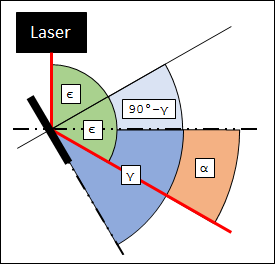
\includegraphics[width=.95\linewidth]{alpha.png}
	\end{minipage}
	\hfill
	\begin{minipage}[c]{0.49\textwidth}
		\centering
		$ \begin{aligned}
			\alpha = f_2(\gamma) & = \epsilon - (\dg{90} - \gamma) \qquad \textit{mit} \quad \epsilon = \dg{90} - (\dg{90} - \gamma) \\
			       & = (\dg{90} - (\dg{90} - \gamma)) - (\dg{90} - \gamma) \\
		           & = \dg{90} - \dg{90} + \gamma - \dg{90} + \gamma \\
		           & = 2\gamma - \dg{90}
		\end{aligned} $
	\end{minipage}
	\caption*{b) Berechnung $\alpha$}
\end{figure}

\begin{itemize}[itemsep=0pt]
	\item $f_2(\dg{45}) = 2 \cdot \dg{45} - \dg{90} =  \dg{0}$
	\item $f_2(\dg{77}) = 2 \cdot \dg{77} - \dg{90} =  \dg{64}$
\end{itemize}


\subsection{Stellen Sie die Gleichung $z = f_3(\alpha, \beta)$ auf, um aus den Winkeln $\alpha$ und $\beta$ den Tiefenwert $z$ zu berechnen. \\ Welcher Tiefenwert gehört zu den Winkeln $\alpha = 15^\circ$ und $\beta = 30^\circ$?}

\begin{figure}[H]
	\centering
	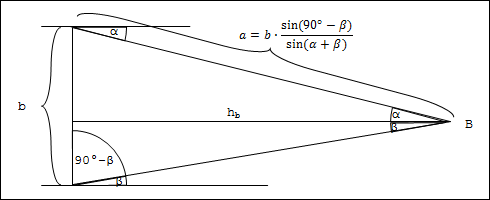
\includegraphics[width=.95\linewidth]{z.png}
	\caption*{c) Berechnung $z$}
\end{figure}

Mithilfe des Sinussatzes gilt: $$ a = b \cdot \frac{\sin(\dg{90} - \beta)}{\sin(\alpha + \beta)} $$
Weiter gilt: $$ \cos(\alpha) = \frac{h_b}{a} $$
Mit $h_b := z$ gilt:
$$ z = f_3(\alpha, \beta) = \cos(\alpha) \cdot \frac{b \cdot \sin(\dg{90} - \beta)}{\sin(\alpha + \beta)} $$
Für $\alpha = \dg{15}$ und $\beta = \dg{30}$ folgt:
$$ z =  f_3(\dg{15}, \dg{30}) = \cos(\dg{15}) \cdot \frac{150mm \cdot \sin(\dg{90} - \dg{30})}{\sin(\dg{15} + \dg{30})} = 177.4519mm $$

\subsection{Stellen Sie die Gleichung $x = f_4(\beta, z)$ auf, um aus dem Winkel $\beta$ und $z$ die $x$-Koordinate zu berechnen \\ Berechnen sie $f_4(40^\circ, 100cm)$.}

\begin{align*}
x = f_4(\beta, z) &= \tan(\beta) \cdot z \\
f_4(\dg{40}, 100cm) &= \tan(\dg{40}) \cdot 100cm = 83,91cm
\end{align*}

\subsection{Stellen Sie nun die Gesamtgleichung $(x,z)^T = f_5(p, \gamma)$ auf, um aus der Pixelposition $p$ und dem Winkel $\gamma$ die Koordinaten $(x, z)^T$ des abgetasteten Punktes zu berechnen. Kürzen Sie sich aufhebende tan und atan Funktionen.}
\newcommand{\fone}[1]{\arctan \left(\frac{#1 + 0.5}{4096} - 1 \right)}
\newcommand{\ftwo}[1]{2#1 - \dg{90}}
\newcommand{\fthree}[2]{\cos\left(#1\right) \cdot \frac{150mm \cdot \sin\left(\dg{90} - #2\right)}{\sin\left(#1 + #2\right)}}
\newcommand{\ffour}[2]{\tan\left(#1\right) \cdot #2}
\begin{align*}
f_5(p, \gamma) = \begin{pmatrix} x \\ z \end{pmatrix} &= \begin{pmatrix} f_4\langle f_1(p), f_3[f_2(\gamma), f_1(p)]\rangle \\ f_3[f_2(\gamma), f_1(p)] \end{pmatrix} \\
%&= \begin{pmatrix} \tan\left(f_1(p)\right) \cdot f_3[f_2(\gamma), f_1(p)] \\ f_3[f_2(\gamma), f_1(p)] \end{pmatrix} \\
&= \begin{pmatrix} 
\ffour{f_1(p)}{f_3(f_2(\gamma), f_1(p))} \\
\fthree{f_2(\gamma)}{f_1(p)} \\
\end{pmatrix} \\
&= \begin{pmatrix} 
\ffour{\fone{p}}{\fthree{\ftwo{\gamma}}{\fone{p}}} \\
\fthree{\ftwo{\gamma}}{\fone{p}} \\
\end{pmatrix} \\
&= \begin{pmatrix}
\left(\frac{p + 0.5}{4096} - 1 \right) \cdot \fthree{\ftwo{\gamma}}{\fone{p}} \\
\fthree{\ftwo{\gamma}}{\fone{p}} \\
\end{pmatrix} \\
&= \begin{pmatrix}
\left(\frac{p + 0.5}{4096} - 1 \right) \cdot f_3[f_2(\gamma), f_1(p)] \\ f_3[f_2(\gamma), f_1(p)] \\
\end{pmatrix}
\end{align*}

\subsection{Zum Spiegelwinkel $\gamma = 67^\circ$ wird ein Laserpunkt im Mittelpunkt von Pixel 5730 registriert. Welche Koordinaten hat der abgetastete Punkt mit oben beschriebenen Aufbau?}
$$ f_5(\dg{67}, 5730) = (43.8599, 109.9113)^T $$

\end{document}
